\documentclass{article}

% Language setting
\usepackage[english]{babel}

% Set page size and margins
% Replace `letterpaper' with `a4paper' for UK/EU standard size
\usepackage[letterpaper,top=2cm,bottom=2cm,left=3cm,right=3cm,marginparwidth=1.75cm]{geometry}

% Useful packages
\usepackage{amsmath}
% --- Code listings ---
\usepackage{listings}
\usepackage{xcolor}
\definecolor{codegreen}{rgb}{0,0.6,0}
\definecolor{codegray}{rgb}{0.5,0.5,0.5}
\definecolor{codepurple}{rgb}{0.58,0,0.82}
\definecolor{backcolour}{rgb}{0.95,0.95,0.92}

\lstdefinestyle{mystyle}{
    backgroundcolor=\color{backcolour},   
    commentstyle=\color{codegreen},
    keywordstyle=\color{magenta},
    numberstyle=\tiny\color{codegray},
    stringstyle=\color{codepurple},
    basicstyle=\ttfamily\footnotesize,
    breakatwhitespace=false,         
    breaklines=true,                 
    captionpos=b,                    
    keepspaces=true,                 
    numbers=left,                    
    numbersep=5pt,                  
    showspaces=false,                
    showstringspaces=false,
    showtabs=false,                  
    tabsize=2
}

\lstset{style=mystyle}
% --- End Code Listings
\usepackage{graphicx}
\usepackage{float}
\usepackage{caption}
% \captionsetup{labelformat=empty} 
% \usepackage{subcaption}
\usepackage[colorlinks=true, allcolors=blue]{hyperref}
\graphicspath{{./figures/}}

\title{ECE 637 Lab - Image Halftoning}
\author{Colin Braun}

\begin{document}
\maketitle

\section{Thresholding and Random Noise Binarization}
\subsection{Original image and result of thresholding}
\begin{figure}[H]
    \centering
    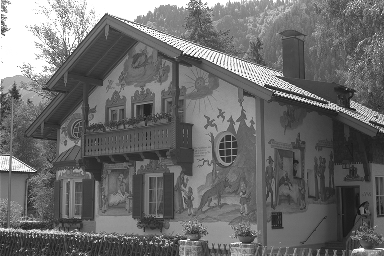
\includegraphics[width=1\textwidth]{../house.png}
    \caption{Original image.}
\end{figure}
\begin{figure}[H]
    \centering
    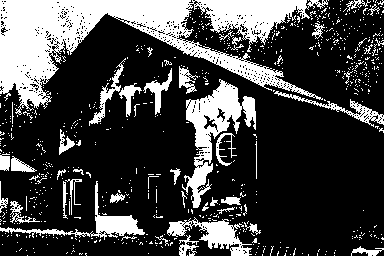
\includegraphics[width=1\textwidth]{../3-thresholded-image.png}
    \caption{BW image after applying threshold}
\end{figure}
\subsection{Computed RMSE and fidelity values}
\subsection{Code for fidelity function}
\lstinputlisting[language=Python, firstline=18, lastline=37]{../section3.py}

\section{Ordered Dithering}
\subsection{The three Bayer index matrices of sizes 2 × 2, 4 × 4, and 8 × 8}
\subsection{The three halftoned images produced by the three dither patterns}
\begin{figure}[H]
    \centering
    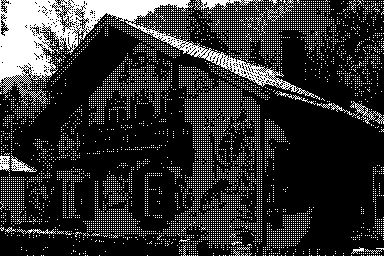
\includegraphics[width=1\textwidth]{../4-b2x2.png}
    \caption{Result using 2x2 index matrix.}
\end{figure}
\begin{figure}[H]
    \centering
    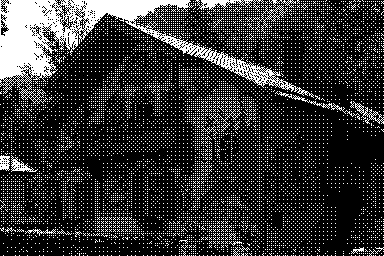
\includegraphics[width=1\textwidth]{../4-b4x4.png}
    \caption{Result using 4x4 index matrix.}
\end{figure}
\begin{figure}[H]
    \centering
    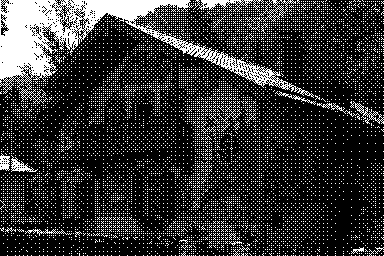
\includegraphics[width=1\textwidth]{../4-b8x8.png}
    \caption{Result using 8x8 index matrix.}
\end{figure}
\subsection{The RMSE and fidelity for each of the three halftoned images}

\section{Error Diffusion}
\subsection{Error diffusion Python code}
\lstinputlisting[language=Python]{../section5.py}
\subsection{Error diffusion result}
\begin{figure}[H]
    \centering
    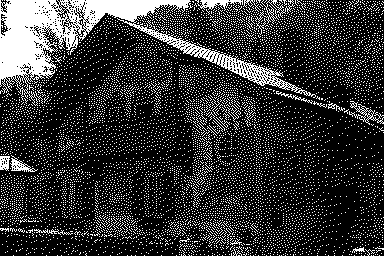
\includegraphics[width=1\textwidth]{../5-diffusion-result.png}
    \caption{The error diffusion result}
\end{figure}
\subsection{The RMSE and fidelity of the error diffusion result}
\subsection{Tabulated RMSE and fidelity results}

\end{document}
